%----------------------------------------------------------------------------------------
  %	PACKAGES AND OTHER DOCUMENT CONFIGURATIONS
  %----------------------------------------------------------------------------------------
  % \RequirePackage{silence}
  % \WarningsOff*
  % \batchmode
  % \documentclass[twoside,twocolumn]{article}
  \documentclass[utf8]{ctexart}
  \raggedbottom
  \usepackage{ctex}
  
  % ======== 通用设置 ========
  
  % 页面布局
  \usepackage{geometry}
  \geometry{a4paper,top=3cm,bottom=3cm,inner=2cm,outer=2cm,marginparwidth=1.8cm}
  
  % 兼容utf8的字体设置
  \setmainfont{CMU Serif}
  % \setCJKmainfont[ItalicFont={华文楷体}]{思源宋体 CN}
  % 思源宋体CN下载:https://github.com/adobe-fonts/source-han-serif/releases/download/2.002R/14_SourceHanSerifCN.zip
  
  % 必备数学套件
  \usepackage{amsmath,amsthm,amsfonts,amssymb}
  \usepackage{bm,bbm,upgreek}
  
  % 图片导入配置
  \usepackage{graphicx}
  \usepackage[export]{adjustbox}
  % 搜寻图片的路径
  \graphicspath{ {./images/} }
  
  % 图注设置
  \usepackage[small,labelfont=bf,up,up,margin=2em]{caption} % Custom captions under/above floats in tables or figures
  
  % 公式、图等的编号设置
  \usepackage{chngcntr}
  %   \counterwithout{figure}{chapter}
  %   \counterwithin{equation}{section}
  
  % 列表设置
  \usepackage{enumitem} % Customized lists
  \setlist[itemize]{itemsep=0pt} % Make itemize lists more compact
  \setlist[enumerate]{itemsep=0pt,parsep=0pt,label={[\arabic*]}}
  
  % 页眉页脚
  \usepackage{fancyhdr}
  \pagestyle{fancy}
  \fancyfoot[EL,OR]{\bfseries· \thepage ·}
  \fancyfoot[C]{}
  \renewcommand{\headrulewidth}{0pt}
  
  % 标题设置
  \usepackage{titling} % Customizing the title section
  % 摘要环境设置(book模板中无效)
  \usepackage{abstract} % Allows abstract customization
  \renewcommand{\abstractnamefont}{\normalfont\bfseries} % Set the "Abstract" text to bold
  \renewcommand{\abstracttextfont}{\normalfont\small\itshape} % Set the abstract itself to small italic text
  
  % 色彩
  \usepackage[svgnames]{xcolor} % added by Wenyin for color
  
  % 超链接设置
  \usepackage[
  colorlinks,
  linkcolor=blue,
  bookmarksnumbered=true,
  bookmarksopen=true
  ]{hyperref}
  % unicode支持:pdf目录可以正确显示公式
  \hypersetup{unicode, psdextra}
  % PDF目录自定义
  \usepackage{bookmark}
  \bookmarksetup{
  	open,
  	numbered,
  	addtohook={%
  		\ifnum\bookmarkget{level}=0 % chapter
  		\bookmarksetup{bold,color=orange}%
  		\fi
  	}
  }
  
  
  
  
  % ======== 可选设置 ========
  
  % for multiple references with dash
  \usepackage[noadjust]{cite}
  \renewcommand{\citedash}{--}    % when \usepackage{cite}
  
  % 额外数学包
  \usepackage{mathrsfs} 	% for \mathscr
  \usepackage{mathtools} 	% for $\intertext{text}$
  \usepackage{breqn}		% 一个可以自动公式断行的公式环境,效果一般
  \usepackage{mhchem} 	%化学式
  \usepackage{esint}
  
  % 表格类
  \usepackage{booktabs} 	% Horizontal rules in tables
  %\usepackage{longtable}	% 长表格
  %\usepackage{tabu}		% 强大的表格包
  %\usepackage{supertabular}
  
  % 杂技
  \usepackage{multirow}	% 多栏布局
  \usepackage{ulem}		% 下划线
  \usepackage{tikz}		% 绘图工具
  \usepackage{framed}		% 文字加框
  \usepackage{setspace}	% 设置行间距等
  \usepackage{minitoc}	% 小目录
  %\usepackage{tcolorbox}	% 多彩盒子工具,巨复杂
  %\tcbuselibrary{skins,breakable,raster}
  \usepackage{float}		% 图片位置:H
  \usepackage{multicol}	% 普通多栏布局
  \usepackage{changepage} % 页面布局调整
  
  % 多文件
  \usepackage{subfiles}
  
  %代码抄录
  \usepackage{shortvrb}
  	% \MakeShortVerb|*		%|*·|*可以直接原文抄录为texttt
  %\usepackage{listings}
  %\lstset{
  	%	language=[LaTeX]TeX,					%语言
  	%	backgroundcolor=\color{yellow!10},			%背景颜色
  	%	basicstyle=\small\ttfamily,				%基本字格式
  	%	keywordstyle=\bfseries\color{purple},		%关键字格式
  	%	commentstyle=\color{gray},				%注释格式
  	%	numbers=left,						%行号
  	%	numberstyle=\ttfamily\small,				%行号格式
  	%	breaklines,							%允许断行
  	%	frame=shadowbox,						%外框线
  	%	escapeinside={<@}{@>},					%逃逸部分,还给Latex编码
  	%	lineskip=0pt,						%行距
  	%	xleftmargin=0.05\linewidth,
  	%	xrightmargin=0.05\linewidth,				%盒子宽度
  	%	morekeywords={rowfont}					%更多自定义关键词
  	%	}
  
  
  
  % 段落分栏包,实现中英对照排版的核心工具
  \usepackage{paracol}
  \setlength{\columnseprule}{0.5pt}
  \setlength{\columnsep}{2em}
  \columnratio{0.4}
  
  
  % ======== 自定义命令 ========
  
  % 数学自定义
  \newcommand{\vect}[1]{\mathbf{\boldsymbol{#1}}} % works for both English and Greek letters, but it does not work with mathtime pro lite fonts, see https://tex.stackexchange.com/questions/3535/bold-math-automatic-choice-between-mathbf-and-boldsymbol-for-latin-and-greek 
  % \newcommand{\matr}[1]{\boldsymbol{\mathrm{#1}}} % \matrix is defined in LaTeX2e kernel
  \newcommand{\tens}[1]{\boldsymbol{\mathrm{#1}}}
  \newcommand\ii{\symup{i}}
  \newcommand\ee{\symup{e}}
  \newcommand\dd{\symup{d}}
  \newcommand\ppi{\symup{\pi}}	%常用的正体字符:i,e,d,\pi
  
  \renewcommand{\paragraph}[1]{\textbf{#1}}
  % ====== 对照排版的设置 ======
  
  % ===中英文对照排版,四六开===
  \columnratio{0.4}
  \newcommand\mainskip{-5pt}
  \newcommand\enzhbox[2]{
  	\quad\par \begin{paracol}{2} \colseprulecolor{black} 
  		\begin{spacing}{1.0}
  			\footnotesize  #1
  		\end{spacing}
  		\switchcolumn[1] 
  		#2
  	\end{paracol} \quad\par
  }
  
  % ===中英文对照排版,五五开===
  %\columnratio{0.48}
  %\newcommand\mainskip{-5pt}
  %\newcommand\enzhbox[2]{
  %	\quad\par \begin{paracol}{2} \colseprulecolor{black} 
  %		\begin{spacing}{1.0}
  %			\small  #1
  %		\end{spacing}
  %		\switchcolumn[1] 
  %		#2
  %	\end{paracol} \quad\par
  %}
  
  % === 仅英文(#1)/仅中文(#2) ===
  % \newcommand\mainskip{5pt}
  % \newcommand\enzhbox[2]{#1}
  %\newcommand\enzhbox[2]{#2}
  
  %%编号层级表
  %%-1 part
  %%0 chapter
  %%1 section
  %%2 subsection
  %%3 subsubsection
  %%4 paragraph
  %%5 subparagraph
  % % 章节标题编号深度
  % \setcounter{secnumdepth}{3}		
  % % 目录深度
  % \setcounter{tocdepth}{2}
  % % 小目录深度
  % \setcounter{minitocdepth}{3}
  % \renewcommand\mtctitle{本章目录}
  
  %----------------------------------------------------------------------------------------
  %	TITLE SECTION
  %----------------------------------------------------------------------------------------
  
  % \setlength{\droptitle}{-4\baselineskip} % Move the title up
  
  % \pretitle{\begin{center}\Huge\bfseries} % Article title formatting
  % 	\posttitle{\end{center}} % Article title closing formatting
 \title{压强和电感效应对异形托卡马克垂直稳定性的影响\\ \Large{PRESSURE AND INDUCTANCE EFFECTS ON THE VERTICAL STABILITY OF SHAPED TOKAMAKS }}  \author{D.J. WARD,  A. BONDESON,  F. HOFMANN et al.}
  
  \newcommand\paperref{D.J. WARD. 1993 Nucl. Fusion 33 821}
   
  \date{\paperref}
  \fancyhead[C]{\small \paperref}
  \fancyhead[L,R]{}
  \renewcommand\headrulewidth{0.6pt}
  \renewcommand{\maketitlehookd}{%
  	\begin{abstract}
 {本文给出了数值计算结果,以展示压强和电感对异形托卡马克垂直稳定性的影响。较高的 $\epsilon \beta_{p}$ 值可改善 D 形托卡马克的垂直稳定性,但会使反 D 形托卡马克失稳。对于拉长截面,稳定的内部电感 $l_{\mathrm{i}}$ 的最大值与 $\epsilon \beta_{\mathrm{p}}$ 呈线性关系,很好地描述了压强效应,其系数取决于几何形状并随三角形变增大。文中给出了类似 TCV 和 DIII - D 截面的 $l_{\mathrm{i}}$ 与 $\epsilon \beta_{\mathrm{p}}$ 的稳定性图。电流剖面效应严重依赖于壁的位形:若壁较近,较低的 $l_{\mathrm{j}}$ 值可使系统稳定,但在无壁的情况下会增加不稳定性的驱动力。对于具有离散外部导体的位形,本文考虑了这两种效应之间的竞争。 
}\\ \indent  Numerical calculations are presented to show the influence of pressure and inductance on the vertical stability of shaped tokamaks. High values of $\epsilon \beta_{p}$ improve the vertical stability of dee shaped tokamaks but are destabilizing for an inverse dee. For elongated cross-sections, the pressure effect is well described by a linear dependence of the maximum value of the stable internal inductance $l_{\mathrm{i}}$ on $\epsilon \beta_{\mathrm{p}}$, with a coefficient that depends on the geometry and increases with the triangularity. Stability diagrams are shown in terms of $l_{\mathrm{i}}$ versus $\epsilon \beta_{\mathrm{p}}$ for TCV- and DIII-D-like crosssections. Current profile effects depend critically on the wall configuration: low values of $l_{\mathrm{j}}$ are stabilizing if the wall is close, but increase the driving force of the instability in the absence of a wall. The competition between these two effects is considered for a configuration with discrete external conductors.
  	\end{abstract}
  }
  
  %----------------------------------------------------------------------------------------
  
  \begin{document}
  \begin{sloppypar}
  	% \nonstopmode 
  	% \WarningsOff[latex] 
  % 公式环境的一些设置
  \allowdisplaybreaks[3]  
  \setlength{\abovedisplayskip}{-6pt}
  \setlength{\belowdisplayskip}{10pt}
  \setlength{\abovedisplayshortskip}{0pt}
  \setlength{\belowdisplayshortskip}{0pt}
  \setlength{\parskip}{\mainskip}
  
  	% \setcounter{chapter}{3}
  	\maketitle
 
 {\centering \textbf{AI总结} \par}
 \begin{adjustwidth}{0.1\linewidth}{0.1\linewidth} \small  \setlength{\parskip}{2pt}
 该论文聚焦于压强和电感效应对异形托卡马克垂直稳定性的影响,通过数值计算和理论分析得出了一系列重要结论,具体内容如下:

1. \textbf{研究背景}:现代托卡马克利用拉长截面提升性能,但拉长会引发垂直不稳定性,这限制了可实现的拉长比,因此研究垂直稳定性的运行极限及其影响因素至关重要。

2. \textbf{稳定性图分析}

• \textbf{TCV和DIII - D截面}:通过数值计算给出了TCV和DIII - D截面的垂直稳定性图,发现临界内部电感$l_{\mathrm{i}, \text { crit }}$近似是$\epsilon \beta_{\mathrm{p}}$的线性函数,与电流剖面细节和环径比无关,但对截面几何形状和到壁的距离敏感。对于常见的D形,压强具有稳定作用;在反D形中,压强会导致失稳。

• \textbf{不同形状对比}:三角形变会增大$l_{\mathrm{i}, \text { crit }}$随$\epsilon \beta_{\mathrm{p}}$变化的斜率,拉长比会减小该斜率,在比较DIII - D和TCV D形时,三角形变的影响占主导地位。

3. \textbf{理论结果回顾}:前人通过解析、半解析或数值方法对形状、压强和电感对垂直稳定性的影响进行了研究,表明拉长会使垂直位移失稳,导电壁可实现稳定,有限压强与正三角形变共同作用对拉长平衡态的垂直稳定性具有稳定效应。

4. \textbf{压强效应}

 • \textbf{不同形状表现}:压强对D形的主要影响是降低自由空间驱动能量,对反D形则增加自由空间能量,对椭圆形,自由空间增长率不受压强影响,但高压时壁致稳作用增强。

  • \textbf{与三角形变关系}:压强效应与三角形变密切相关,反D形中压强致失稳,标准D形中压强致稳定。

5. \textbf{电流剖面效应}

 • \textbf{对垂直稳定性影响}:电流剖面强烈影响垂直稳定性,低内部电感的平坦电流剖面增强等离子体与外部导体的耦合,但无导电壳时,增长率随电感减小而增大。

  • \textbf{壁间距的作用}:壁较远时,电流剖面峰化具有稳定作用;壁较近时,峰化导致失稳。内部电感对理想壁临界位置影响小,对紧密贴合壁的电阻增长率影响大。

6. \textbf{离散导体的被动致稳}:离散导体替代完整包围壁时,电流剖面展宽导致的失稳力增加占主导,增长率随$l_{\mathrm{i}}$减小而增大;而封闭壁位形下,增长率随$l_{\mathrm{i}}$减小而单调降低。

7. \textbf{研究结论}:较高的$\epsilon \beta_{\mathrm{p}}$值显著改善D形托卡马克的垂直稳定性,临界内部电感与$\epsilon \beta_{\mathrm{p}}$近乎线性相关,系数$c$随三角形变增大、随拉长比减小。这种效应有利于达到高比压。  \end{adjustwidth}   \setlength{\parskip}{\mainskip}
 
  % ==document boby begins
  
  
 \section{引言}
 {  \small INTRODUCTION \par }
 
\enzhbox{  Modern tokamaks are generally designed so as to take advantage of the increased current capability of an elongated cross-section and the resulting improvement of the beta limit \textcolor{green!50!black}{[1,2]} and confinement time \textcolor{green!50!black}{[3]}. A well known drawback of elongation is vertical instability $\textcolor{green!50!black}{[4,5]}$, which requires the use of conducting walls close to the plasma assisted by active feedback stabilization on the $L / R$ time-scale of the resistive wall. Work on the DIII-D tokamak has established that vertical instability is the factor that limits the achievable elongation \textcolor{green!50!black}{[2, 6]}. For the TCV experiment \textcolor{green!50!black}{[7]} in Lausanne, designed for a maximum elongation of $\kappa=3$, the vertical stability is a major issue, and we have therefore investigated numerically the operational limits due to the vertical instability and how these depend on, e.g., the shape of the plasma cross-section and the equilibrium profiles.}{
现代托卡马克通常设计成利用拉长截面所增加的电流承载能力,以及由此带来的比压极限 \textcolor{green!50!black}{[1,2]} 和约束时间 \textcolor{green!50!black}{[3]} 的改善。拉长的一个众所周知的缺点是垂直不稳定性 \textcolor{green!50!black}{[4,5]},这需要在等离子体附近使用导电壁,并在电阻壁的 $L / R$ 时间尺度上借助主动反馈稳定系统。DIII - D 托卡马克的研究已经证实,垂直不稳定性是限制可实现拉长比的因素 \textcolor{green!50!black}{[2, 6]}。对于洛桑的 TCV 实验 \textcolor{green!50!black}{[7]},其设计的最大拉长比 $\kappa = 3$,垂直稳定性是一个主要问题。因此,我们通过数值方法研究了由垂直不稳定性导致的运行极限,以及这些极限如何依赖于例如等离子体截面形状和平衡剖面等因素。 }
  
 
\enzhbox{  It is found experimentally \textcolor{green!50!black}{[8]} that the vertical stability of strongly elongated tokamaks is favoured by a low internal inductance $l_{\mathrm{i}}$, because this increases the coupling of the plasma current to the surrounding wall. Vertical stability requires an internal inductance less than some threshold value $l_{\mathrm{i}, \text { crit }}$, which decreases with increasing elongation and wall distance. Here, we mean by $l_{\mathrm{i}, \text { crit }}$ the value of $l_{\mathrm{i}}$ for which a plasma surrounded by a realistic resistive wall has an $n=0$ growth rate, $\gamma_{\text {crit }}$, below which the vertical position can be controlled by a practical feedback system.}{
实验发现 \textcolor{green!50!black}{[8]},强拉长托卡马克的垂直稳定性得益于较低的内部电感 $l_{\mathrm{i}}$,因为这会增强等离子体电流与周围壁的耦合。垂直稳定性要求内部电感小于某个阈值 $l_{\mathrm{i}, \text { crit }}$,该阈值随拉长比和壁间距的增加而减小。这里,我们所说的 $l_{\mathrm{i}, \text { crit }}$ 是指对于被实际电阻壁包围的等离子体,其 $n = 0$ 增长率为 $\gamma_{\text {crit }}$ 时对应的 $l_{\mathrm{i}}$ 值,在该增长率以下,垂直位置可由实际的反馈系统控制。 }
  
  
 
\enzhbox{  Our principal result is that $l_{\mathrm{i}, \text { crit }}$ is strongly influenced by pressure in combination with triangular shaping of the cross-section. We find numerically that $l_{i, \text { crit }}$ is an approximately linear function of $\epsilon \beta_{\mathrm{p}}$, independent of the details of the current profile and aspect ratio, but sensitively dependent on the geometry of the crosssection and the distance to the wall. For the usual dee shape, pressure is stabilizing, i.e. $l_{\mathrm{i} \text {, crit }}$ increases with $\epsilon \beta_{\mathrm{p}}$, whereas in an inverse dee, pressure is destabilizing. The increased upper limit in internal inductance for a normal dee is a favourable effect, not only because it makes it possible to reach a higher elongation, but also because the beta limit $\textcolor{green!50!black}{[2,9]}$ and confinement time \textcolor{green!50!black}{[10]} improve with the internal inductance at fixed elongation. Reference \textcolor{green!50!black}{[2]} shows convincing evidence that the optimum condition for reaching high beta is at the intersection of the $n=0$ and $n=1$ stability boundaries, where $n$ is the toroidal mode number.}{
我们的主要结果是,$l_{\mathrm{i}, \text { crit }}$ 受压强以及截面的三角形变共同影响显著。我们通过数值计算发现,$l_{i, \text { crit }}$ 近似是 $\epsilon \beta_{\mathrm{p}}$ 的线性函数,与电流剖面细节和环径比无关,但对截面几何形状和到壁的距离十分敏感。对于常见的 D 形,压强具有稳定作用,即 $l_{\mathrm{i} \text {, crit }}$ 随 $\epsilon \beta_{\mathrm{p}}$ 增大而增大,而在反 D 形中,压强会导致失稳。对于正常 D 形,内部电感上限的提高是一个有利影响,这不仅是因为它使得能够达到更高的拉长比,还因为在固定拉长比的情况下,比压极限 \textcolor{green!50!black}{[2,9]} 和约束时间 \textcolor{green!50!black}{[10]} 会随内部电感的增加而改善。文献 \textcolor{green!50!black}{[2]} 给出了令人信服的证据,表明达到高比压的最优条件是在 $n = 0$ 和 $n = 1$ 稳定性边界的交点处,其中 $n$ 是环向模数。 }
  
 
\enzhbox{  The stabilizing effect of low inductance $l_{\mathrm{i}}$ is due to improved wall coupling in configurations with a completely surrounding wall. However, broad current profiles tend to give higher ideal growth rates with the wall at infinity. Here, we shall discuss the competition of these effects for a configuration where the wall is replaced by discrete conductors.}{
低电感 $l_{\mathrm{i}}$ 的稳定效应源于在完全包围等离子体的壁位形中壁耦合的改善。然而,当壁在无穷远处时,宽电流剖面往往会导致更高的理想增长率。在此,我们将讨论在壁被离散导体替代的位形中这些效应之间的竞争。 }
  
 \section{TCV 和 DIII - D 截面的稳定性图}
 {  \small STABILITY DIAGRAMS FOR TCV AND DIII-D CROSS-SECTIONS \par }
 
\enzhbox{  Figure 1 shows the limit in internal inductance $l_{\mathrm{i}, \text {, rit }}$ as a function of $\epsilon \beta_{p}$ for three different classes of current profiles in a 'TCV cross-section' at aspect ratio $A=1 / \epsilon=R_{0} / a=3.7$ (curves $1-3$ ). The following definitions are used for the poloidal beta:}{
\textcolor{blue}{图 1} 展示了在环径比 $A = 1 / \epsilon=R_{0} / a = 3.7$ 的 “TCV 截面” 中,针对三类不同的电流剖面,内部电感极限 $l_{\mathrm{i}, \text { crit }}$ 随 $\epsilon \beta_{p}$ 的变化情况(曲线 1 - 3)。极向比压的定义如下:}
 \begin{align*}
 	 \beta_{\mathrm{p}} \equiv \frac{4}{\mu_{0} I_{\mathrm{p}}^{2} R_{0}} \int_{\mathrm{pt}} p \mathrm{~d}^{3} x
 \end{align*}
  
 
\enzhbox{  \noindent and internal inductance}{
\noindent 以及内部电感}
  \begin{align*}
  l_{\mathrm{i}} \equiv \frac{2}{\mu_{0}^{2} I_{\mathrm{p}}^{2} R_{0}} \int_{\mathrm{p} \ell} B_{\mathrm{p}}^{2} \mathrm{~d}^{3} x
  \end{align*}
  
 
\enzhbox{  The plasma-vacuum boundary is specified as}{
等离子体 - 真空边界定义如下}
  \begin{gather*}
  	R / a=A+\cos (\theta+\delta \sin \theta+\lambda \sin 2 \theta) \tag{1}\\
  Z / a=\kappa \sin \theta 
  \end{gather*}
  
  
 
  
 
\enzhbox{  \noindent and the geometry referred to as 'TCV dee' has elongation $\kappa=3$, triangularity $\delta=0.5$ and squareness $\lambda=0.2$. Equilibria have been computed with the CHEASE code \textcolor{green!50!black}{[11]} and stability with the NOVA-W code \textcolor{green!50!black}{[12]}, which is capable of computing the growth rates of $n=0$ modes with a resistive wall, as well as with an ideal wall or with no wall. Figure 1 refers to resistive wall instabilities (cases that are stable with an ideal wall), and it is assumed that the mode can be stabilized by active feedback control if the resistive wall growth time is longer than $7 \%$ of the $L / R$ time of the wall (more precisely, for its ' $m=1$ ' eigenmode), i.e. 0.5 ms . The conducting wall represents the TCV vacuum vessel \textcolor{green!50!black}{[7]}.}{
\noindent 并且被称为 “TCV D 形” 的几何形状具有拉长比 $\kappa = 3$、三角形变 $\delta = 0.5$ 和矩形比 $\lambda = 0.2$。已使用 CHEASE 程序 \textcolor{green!50!black}{[11]} 计算平衡态,使用 NOVA - W 程序 \textcolor{green!50!black}{[12]} 计算稳定性,NOVA - W 程序能够计算存在电阻壁、理想壁或无壁情况下 $n = 0$ 模的增长率。\textcolor{blue}{图 1} 涉及电阻壁不稳定性(在理想壁情况下稳定的情况),并且假设如果电阻壁增长时间长于壁的 $L / R$ 时间(更准确地说,是其 “$m = 1$” 本征模)的 7\%,即 0.5 ms,则该模可通过主动反馈控制实现稳定。导电壁代表 TCV 真空室 \textcolor{green!50!black}{[7]}。 }
  \begin{figure}[H]
  	\centering
  	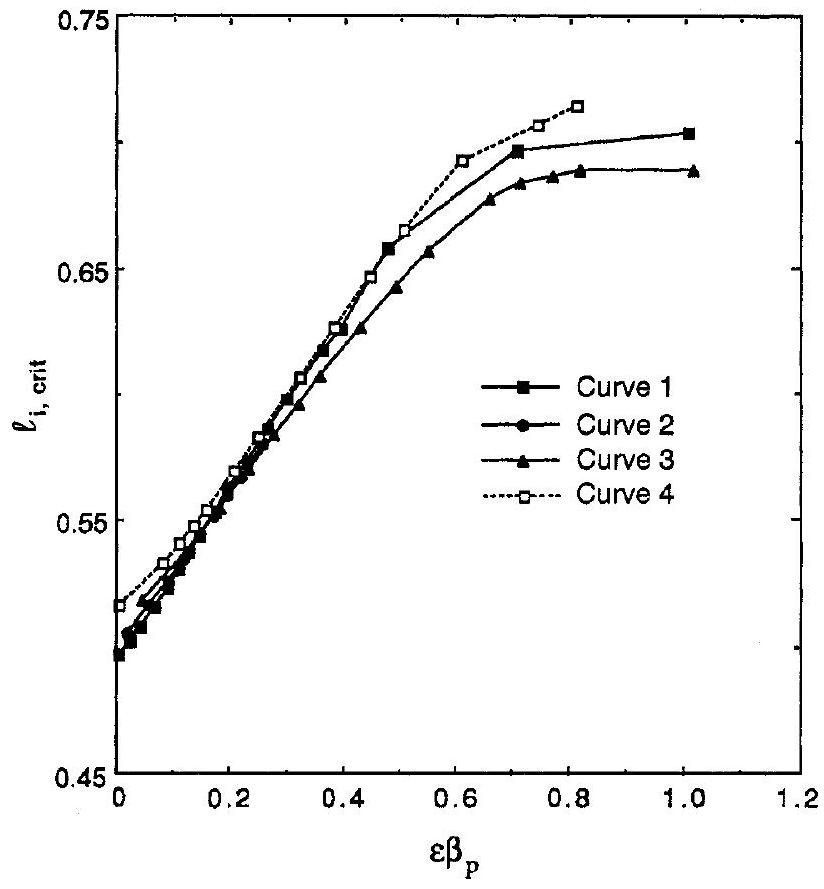
\includegraphics[max width=0.85\textwidth,max height=0.3\textheight]{2025_01_10_a0135324997886412d98g-3}
 \caption{\uline{Vertical stability diagram in terms of $1_{i, \text { crit }}$ and $\epsilon \beta_{p}$ for the TCV configuration. Curves $1-3$ show the results for the standard TCV configuration for three different types of current profiles. Curve 4 shows the results for the TCV plasma and wall shape expanded to an aspect ratio of $\mathrm{R}_{0} / \mathrm{a}=7.0$ for the first current profile.\\}\\TCV 位形下以 $l_{i, \text { crit }}$ 和 $\epsilon \beta_{p}$ 表示的垂直稳定性图。曲线 1 - 3 展示了标准 TCV 位形下三种不同类型电流剖面的结果。曲线 4 展示了将 TCV 等离子体和壁形状扩展到环径比 $\mathrm{R}_{0} / \mathrm{a}=7.0$ 时,第一种电流剖面的结果。}
  	\label{fig1.}
  \end{figure}
  
   % ==AUTO MOVED 
  
 
\enzhbox{  Several conclusions can be drawn from Fig. 1. Firstly, the limit in $l_{\mathrm{i}}$ is the same function of $\beta_{\mathrm{p}}$ for the three different classes of current profiles. The three current profiles differ significantly, and Fig. 2 shows the profiles 1 and 3 for the surface averaged toroidal current density $I^{*}$ at the point $l_{\mathrm{i}}=l_{\mathrm{i}, \text { crit }}$ at low and high pressures ( $\epsilon \beta_{\mathrm{p}}=0$ and 0.5 , respectively). (The pressure profiles have been chosen as uniformly scaled versions of those that give the ballooning limit with a given $I^{*}$ profile.) Secondly, curve 4 refers to an equilibrium with a larger aspect ratio, $A=7$. The large aspect ratio result coincides almost exactly with that for $A=3.7$ when it is plotted in terms of $l_{\mathrm{i}}$ and $\epsilon \beta_{\mathrm{p}}$. Thus, for a fixed, elongated cross-section (but with varying current profile and aspect ratio) $n=0$ stability requires $l_{\mathrm{i}}<l_{\mathrm{i}, \text { crit }}\left(\epsilon \beta_{\mathrm{p}}\right.$ ), and for $\epsilon \beta_{\mathrm{p}}$ not too large $l_{\mathrm{i}, \text { crit }}$ is almost linear in $\epsilon \beta_{\mathrm{p}} ; l_{\mathrm{i}, \text { crit }} \approx l_{\mathrm{i}, 0}+c \epsilon \beta_{\mathrm{p}}$.}{
从\textcolor{blue}{图 1} 可以得出几个结论。首先,对于三种不同类型的电流剖面,$l_{\mathrm{i}}$ 的极限是 $\beta_{\mathrm{p}}$ 的相同函数。这三种电流剖面差异显著,\textcolor{blue}{图 2} 展示了在低压和高压(分别为 $\epsilon \beta_{\mathrm{p}} = 0$ 和 0.5)下,在 $l_{\mathrm{i}} = l_{\mathrm{i}, \text { crit }}$ 处,表面平均环向电流密度 $I^{*}$ 的剖面 1 和剖面 3。(压强剖面被选为那些在给定 $I^{*}$ 剖面下给出气球模极限的压强剖面的均匀缩放版本。)其次,曲线 4 对应于环径比更大($A = 7$)的平衡态。当以 $l_{\mathrm{i}}$ 和 $\epsilon \beta_{\mathrm{p}}$ 为坐标绘图时,大环径比的结果几乎与 $A = 3.7$ 时的结果完全重合。因此,对于固定的拉长截面(但电流剖面和环径比可变),$n = 0$ 稳定性要求 $l_{\mathrm{i}} < l_{\mathrm{i}, \text { crit }}(\epsilon \beta_{\mathrm{p}})$,并且对于不太 大的 $\epsilon \beta_{\mathrm{p}}$,$l_{\mathrm{i}, \text { crit }}$ 与 $\epsilon \beta_{\mathrm{p}}$ 近似呈线性关系;$l_{\mathrm{i}, \text { crit }} \approx l_{\mathrm{i}, 0} + c \epsilon \beta_{\mathrm{p}}$。 }
  
  
 
\enzhbox{  Figure 3 shows the corresponding result for a DIII-D-like cross-section, $\kappa=2.5, \delta=0.6, \lambda=0$ and $A=3$. Here, the resistive wall was chosen to be conformal to the plasma boundary, and two different minor radii have been considered for the wall; $d=1.3 a$ and $d=1.4 a$. The result is similar to that for the TCV dee shape in that the critical internal inductance increases with $\epsilon \beta_{p}$; however, the dependence is much stronger for the DIII-D cross-section. For the DIII-D-like case with $d=1.3 a$, we have $l_{\mathrm{i}, \text { crit }} \approx l_{\mathrm{i}, 0}+c \in \beta_{\mathrm{p}}$, with $c \approx 1.8$, which is much larger than for the TCV dee, where $c \approx 0.34$.}{
\textcolor{blue}{图 3} 展示了类似 DIII - D 截面($\kappa = 2.5$,$\delta = 0.6$,$\lambda = 0$ 且 $A = 3$)的相应结果。在此,电阻壁被选为与等离子体边界共形,并且考虑了壁的两种不同小半径;$d = 1.3a$ 和 $d = 1.4a$。结果与 TCV D 形的情况类似,即临界内部电感随 $\epsilon \beta_{p}$ 增加而增大;然而,对于 DIII - D 截面,这种依赖关系要强得多。对于 $d = 1.3a$ 的类似 DIII - D 情况,我们有 $l_{\mathrm{i}, \text { crit }} \approx l_{\mathrm{i}, 0} + c \epsilon \beta_{\mathrm{p}}$,其中 $c \approx 1.8$,这比 TCV D 形情况($c \approx 0.34$)大得多。 }
  
 
\enzhbox{  Also shown in Fig. 3 are two additional cases that compare the variation of the shape at the two different elongations. The first case has the high elongation ( $\kappa=3$ ) of the TCV dee shape, but with higher triangularity ( $\delta=0.6$ ) and no squareness $(\lambda=0)$. Because of the poor coupling of equilibria with this shape to the TCV vacuum vessel, we use a conformal wall with the distance chosen ( $d=1.275 a$ ) to give the same value of $l_{i, 0}$ as the TCV dee configuration at zero pressure. The stability boundary for this case has a slope almost as large as that for the DIII-D-like crosssection. The other case has the same elongation ( $\kappa=2.5$ ) as the DIII-D-like cross-section, but has the triangularity and squareness parameters corresponding to the TCV dee shape ( $\delta=0.5$ and $\lambda=0.2$ ). This case gives a line with an intermediate slope $c$ which is closer to that of the TCV dee shape. Thus, triangularity increases the slope and elongation decreases it, and in comparing the DIII-D and TCV dee shapes the effect of triangularity is dominant.}{
\textcolor{blue}{图 3} 中还展示了另外两种情况,用于比较两种不同拉长比下形状的变化。第一种情况具有 TCV D 形的高拉长比($\kappa = 3$),但三角形变更高($\delta = 0.6$)且矩形比为零($\lambda = 0$)。由于这种形状的平衡态与 TCV 真空室的耦合较差,我们使用一个共形壁,其距离选择为($d = 1.275a$),以使零压强下的$l_{i, 0}$值与 TCV D 形位形相同。这种情况下的稳定性边界斜率几乎与类似 DIII - D 截面的斜率一样大。另一种情况与类似 DIII - D 截面具有相同的拉长比($\kappa = 2.5$),但三角形变和矩形比参数对应于 TCV D 形($\delta = 0.5$ 和 $\lambda = 0.2$)。这种情况给出的直线斜率$c$处于中间值,更接近 TCV D 形的斜率。因此,三角形变会增大斜率,拉长比会减小斜率,在比较 DIII - D 和 TCV D 形时,三角形变的影响占主导地位。 }
  
 
\enzhbox{  The stability threshold, of course, depends on the assumptions concerning the critical growth rate $\gamma_{\text {crit }}$. If the critical growth rate is changed, the main effect is a uniform shift of $l_{\mathrm{i}, \text { crit }}\left(\epsilon \beta_{\mathrm{p}}\right)$, with only a small effect on the slope $c$. For example, if $\gamma_{\text {crit }}$ for the TCV case, Fig. 1, is increased by $50 \%$ (this relaxes the demands on the feedback system), then the value of $l_{\mathrm{i}, 0}$ increases from 0.494 to 0.519 , while the slope $c$ increases by about $8 \%$. For the DIII-D-like case, if $\gamma_{\text {crit }}$ is increased by $50 \%$ the value of $l_{\mathrm{i}, 0}$ increases considerably, from 0.521 to 0.667 , but the value of the slope $c$ increases by only $3 \%$.\\ Note that Fig. 3 does not apply literally to DIII-D conditions, e.g. with respect to the assumed value of $\gamma_{\text {crit }} \tau_{\text {wall }}$. Furthermore, our definitions of $\beta_{\mathrm{p}}$ and $l_{\mathrm{i}}$ differ from those used in, for example, Ref. \textcolor{green!50!black}{[2]} by a shape dependent factor. For the DIII-D shape our values are smaller by a factor of approximately 1.5 . Improved vertical stability at high $\beta$ has been observed in DIII-D and was attributed to the broader current profiles at high $\beta$ due to a large fraction of bootstrap current \textcolor{green!50!black}{[2]}. Our calculations show that finite $\beta$ also has a direct effect on vertical stability, and this effect is significant for the DIII-D cross-section.}{
当然,稳定性阈值取决于关于临界增长率 $\gamma_{\text {crit }}$ 的假设。如果改变临界增长率,主要影响是 $l_{\mathrm{i}, \text { crit }}(\epsilon \beta_{\mathrm{p}})$ 整体平移,对斜率 $c$ 的影响很小。例如,对于\textcolor{blue}{图 1} 中的 TCV 情况,如果 $\gamma_{\text {crit }}$ 增加 50\%(这降低了对反馈系统的要求),那么 $l_{\mathrm{i}, 0}$ 的值将从 0.494 增加到 0.519,而斜率 $c$ 仅增加约 8\%。对于类似 DIII - D 的情况,如果 $\gamma_{\text {crit }}$ 增加 50\%,$l_{\mathrm{i}, 0}$ 的值会大幅增加,从 0.521 增加到 0.667,但斜率 $c$ 的值仅增加 3\%。

请注意,\textcolor{blue}{图 3} 并非严格适用于 DIII - D 的条件,例如关于 $\gamma_{\text {crit }} \tau_{\text {wall }}$ 的假设值。此外,我们对 $\beta_{\mathrm{p}}$ 和 $l_{\mathrm{i}}$ 的定义与例如文献 \textcolor{green!50!black}{[2]} 中使用的定义相差一个与形状有关的因子。对于 DIII - D 形状,我们的值大约小 1.5 倍。在 DIII - D 中观察到高 $\beta$ 下垂直稳定性得到改善,并归因于高 $\beta$ 时由于自举电流占比大而导致的更宽的电流剖面 \textcolor{green!50!black}{[2]}。我们的计算表明,有限的 $\beta$ 对垂直稳定性也有直接影响,并且这种影响对于 DIII - D 截面是显著的。 }
  \begin{figure}[H]
  	\centering
  	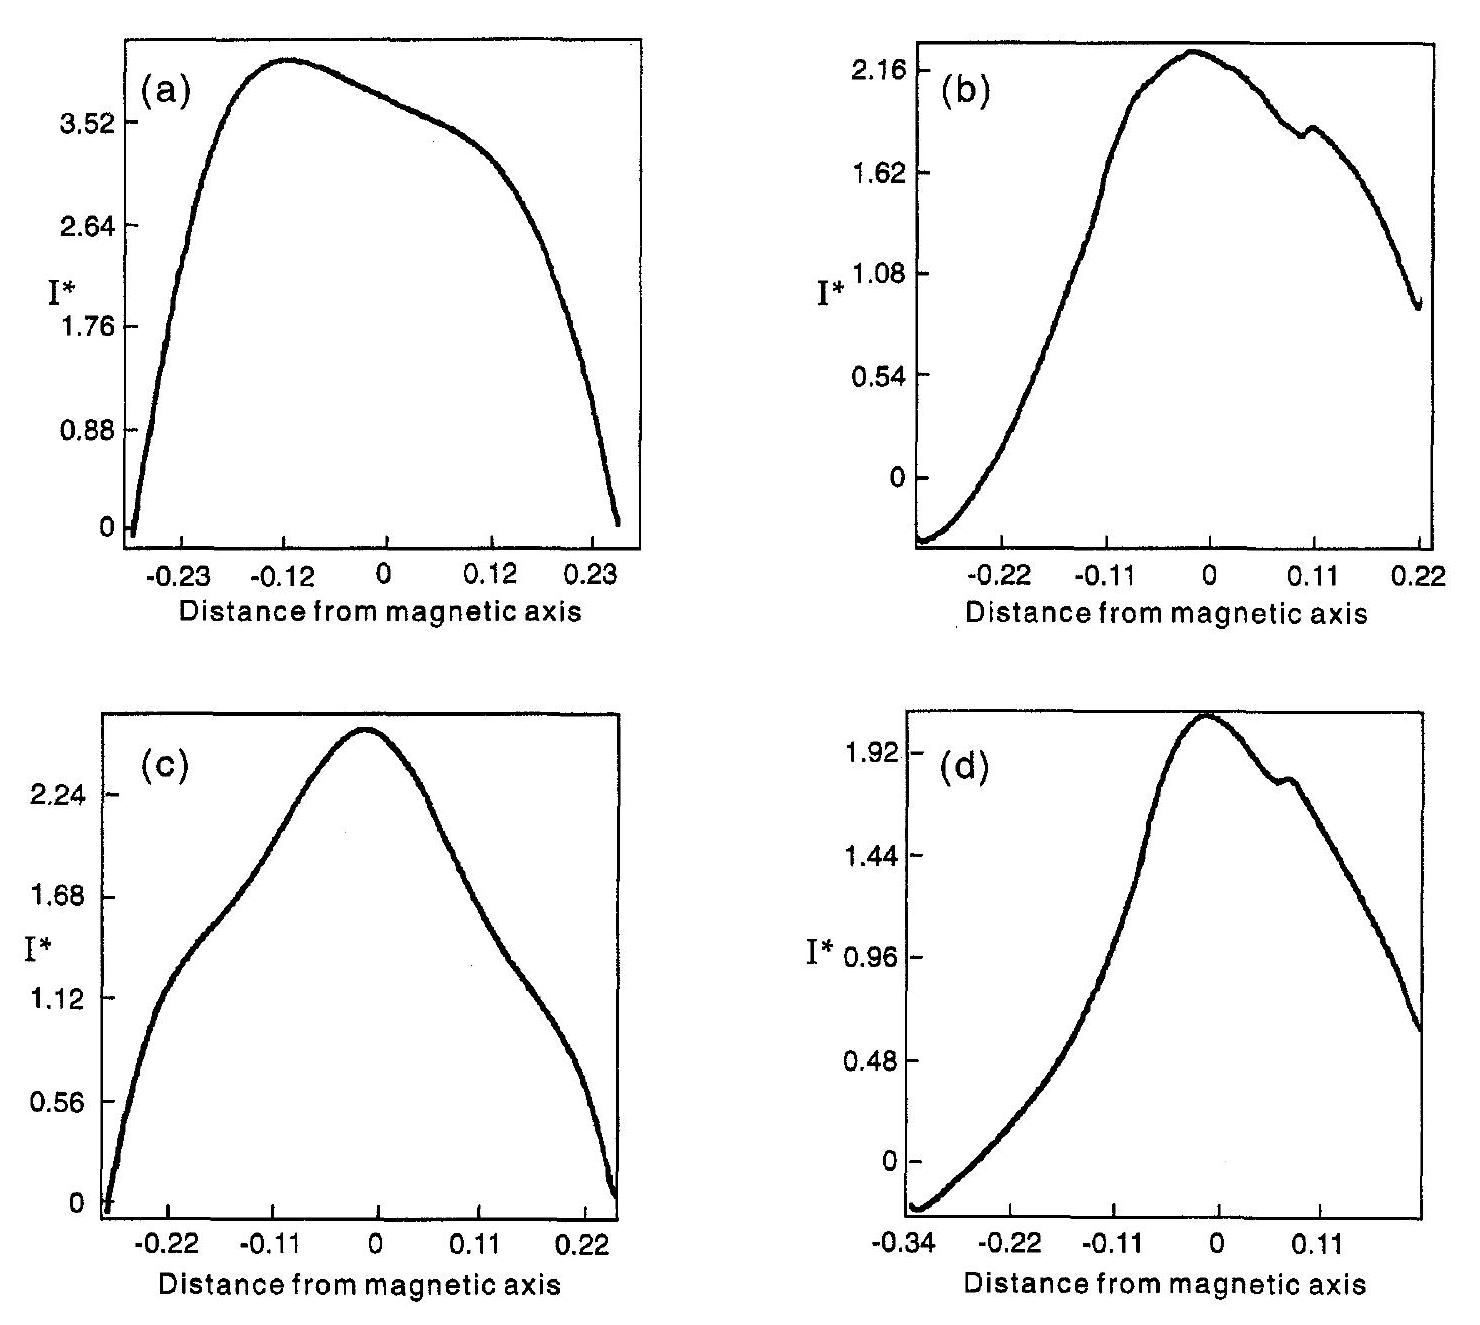
\includegraphics[max width=0.85\textwidth,max height=0.35\textheight]{2025_01_10_a0135324997886412d98g-4}
 \caption{\uline{Current profiles ( 1 * is the surface averaged toroidal current density) corresponding to curves 1 and 3 of Fig. 1. Both profile types are shown at low and high beta: (a) curve $1, \beta_{p}=0.06$; (b) curve $1, \beta_{p}=0.6$; (c) curve 3, $\beta_{p}=0.06$; (d) curve 3, $\beta_{p}=0.6$.}\\对应于\textcolor{blue}{图 1} 中曲线 1 和曲线 3 的电流剖面($I^{*}$ 是表面平均环向电流密度)。两种剖面类型均展示了低比压和高比压情况:(a) 曲线 1,$\beta_{p}=0.06$;(b) 曲线 1,$\beta_{p}=0.6$;(c) 曲线 3,$\beta_{p}=0.06$;(d) 曲线 3,$\beta_{p}=0.6$。 }
  	\label{fig2.}
  \end{figure}
  
   
  % ==AUTO MOVED 
  
 \section{理论结果简要回顾}
 {  \small BRIEF REVIEW OF THEORETICAL RESULTS \par }
 
\enzhbox{  Several results relevant to the diagrams in Figs 1 and 3 have been obtained previously by analytical [ $4,5,13-15]$, semi-analytical \textcolor{green!50!black}{[16, 17]} or numerical \textcolor{green!50!black}{[18-20]} methods. Quite surprisingly, most of the work on shape, pressure and inductance effects on vertical stability dates from the 1970 s, despite the subsequent development of powerful numerical codes and the fact that experiments are now in regimes where such effects are of importance.\\ Zakharov \textcolor{green!50!black}{[4]} showed that vertical elongation, $\kappa>1$, destabilizes vertical shifts but that a weakly elongated equilibrium can be stabilized by finite aspect ratio effects without the use of a conducting shell. Vertical displacements are stable if the decay index $n$ of the external vertical field satisfies $n \equiv-\left(R_{0} / B_{z}^{\text {ext }}\right)\left(\partial B_{z}^{\text {ext }} / \partial R\right)_{R=R_{0}}>0$.}{
先前已通过解析方法 [4,5,13 - 15]、半解析方法 \textcolor{green!50!black}{[16, 17]} 或数值方法 [18 - 20] 得到了几个与\textcolor{blue}{图 1} 和\textcolor{blue}{图 3} 中的图表相关的结果。相当令人惊讶的是,尽管随后开发出了强大的数值程序,并且如今实验已进入这些效应十分重要的状态,但大多数关于形状、压强和电感对垂直稳定性影响的研究可追溯到 20 世纪 70 年代。

扎哈罗夫 \textcolor{green!50!black}{[4]} 表明,垂直拉长($\kappa>1$)会使垂直位移失稳,但弱拉长的平衡态可以在不使用导电壳的情况下,通过有限环径比效应实现稳定。如果外部垂直场的衰减指数 $n$ 满足 $n \equiv-\left(R_{0} / B_{z}^{\text {ext }}\right)\left(\partial B_{z}^{\text {ext }} / \partial R\right)_{R=R_{0}}>0$,则垂直位移是稳定的。 }
  \begin{figure}[H]
  	\centering
  	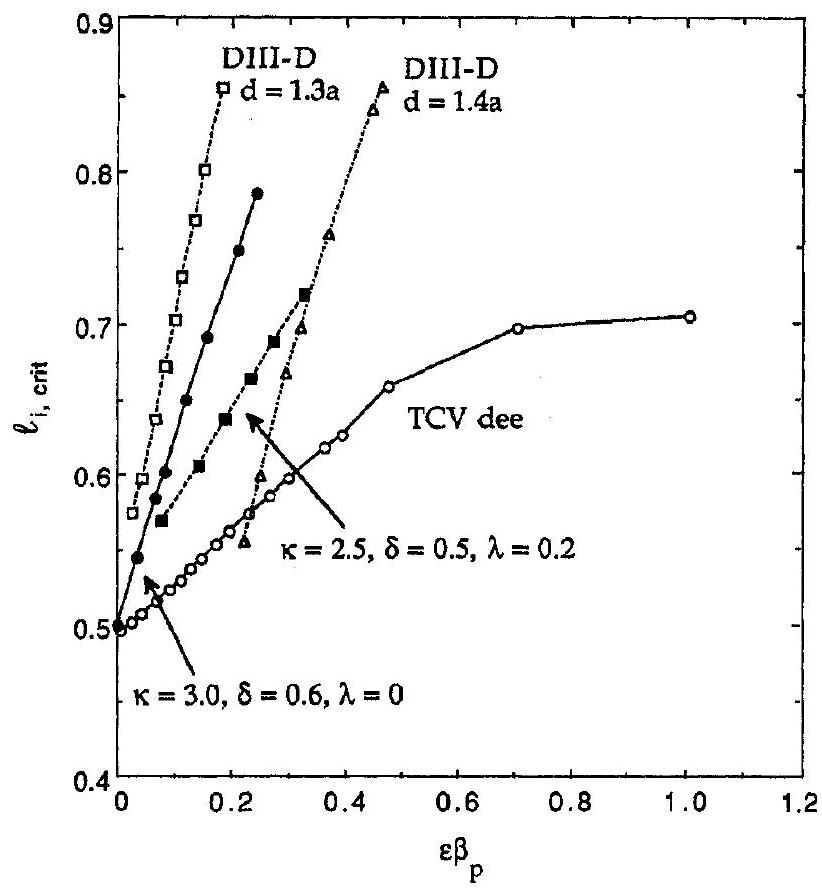
\includegraphics[max width=0.85\textwidth,max height=0.3\textheight]{2025_01_10_a0135324997886412d98g-5}
 \caption{\uline{Vertical stability diagram in terms of $1_{i, \text { crit }}$ and $\epsilon \beta_{p}$ for several equilibria of varying shapes. Two curves are shown for the DIII-D-like equilibrium with two different wall positions. The walls are conformal to the plasma shape at midplane distances of $\mathrm{d}=1.3 \mathrm{a}$ and $\mathrm{d}=1.4 \mathrm{a}$. For comparison, curve 1 from Fig. 1 for the TCV dee configuration is also shown. Two other stability boundaries intermediate between the DIII-D-like and the TCV dee equilibria are shown, with $\kappa=3.0, \delta=0.6, \lambda=0$ and with $\kappa=2.5, \delta=0.5, \lambda=0.2$.}\\几种不同形状平衡态下以 $l_{i, \text { crit }}$ 和 $\epsilon \beta_{p}$ 表示的垂直稳定性图。对于类似 DIII - D 的平衡态,展示了两条对应不同壁位置的曲线。壁在中平面处与等离子体形状共形,距离分别为 $\mathrm{d}=1.3 \mathrm{a}$ 和 $\mathrm{d}=1.4 \mathrm{a}$。为作对比,还展示了\textcolor{blue}{图 1} 中 TCV D 形位形的曲线 1。另外还展示了两条介于类似 DIII - D 和 TCV D 形平衡态之间的稳定性边界,分别对应 $\kappa=3.0$,$\delta=0.6$,$\lambda=0$ 和 $\kappa=2.5$,$\delta=0.5$,$\lambda=0.2$ 的情况。 }
  	\label{fig3.}
  \end{figure}
  
   
  % ==AUTO MOVED 
  
 
\enzhbox{  Zakharov's expression \textcolor{green!50!black}{[4,5]} for $n$ implies that a plasma with a flat current profile is vertically stable when}{
扎哈罗夫 \textcolor{green!50!black}{[4,5]} 给出的关于 $n$ 的表达式表明,具有平坦电流剖面的等离子体在……时是垂直稳定的。(原句未完整,翻译到“when”处) }
 \begin{align*}
 	 \kappa-1<\left(\frac{a}{R_{0}}\right)^{2}\left(\frac{3}{4} \ln \frac{8 R_{0}}{a}-\frac{17}{16}\right) \tag{2}
 \end{align*}
 
\enzhbox{  Laval et al. \textcolor{green!50!black}{[13]} showed that an elongated plasma can be stabilized by a conducting wall. For a flat current profile, their stability condition (in the near circular approximation) is}{
拉瓦尔等人 \textcolor{green!50!black}{[13]} 表明,拉长的等离子体可通过导电壁实现稳定。对于平坦电流剖面,他们的稳定性条件(在近圆形近似下)为……(原句未完整,翻译到“is”处) }
  
 \begin{align*}
 	 \kappa-1<2\left(\frac{a}{d}\right)^{2} \tag{3}
 \end{align*}
  
 
\enzhbox{  \noindent where $d$ is the wall radius. Comparison of the conditions (2) and (3) shows that for the elongations, aspect ratios and wall distances typical of modern tokamaks, wall stabilization is far more important than finite aspect ratio effects \textcolor{green!50!black}{[21]}, and the discharges would be strongly unstable without a wall.}{
\noindent 其中 $d$ 是壁的半径。对比条件 (2) 和 (3) 可知,对于现代托卡马克典型的拉长比、环径比和壁间距而言,壁致稳远比有限环径比效应重要 \textcolor{green!50!black}{[21]},并且若无壁,放电将会是强不稳定的。 }
  
  
 
\enzhbox{  The effects of more complex shaping, including finite aspect ratio and pressure effects, were investigated semi-analytically for a surface current distribution by Rebhan and Salat \textcolor{green!50!black}{[17]}. For vertically elongated equilibria, they found that an inverse dee ( $\delta<0$ ) is destabilized by pressure, but a standard dee ( $\delta>0$ ) can be stabilized by pressure (see Fig. 4(a) of Ref. \textcolor{green!50!black}{[17]}). A stabilizing effect of finite pressure in combination with positive triangularity on the vertical stability of elongated equilibria is also indicated by the results \textcolor{green!50!black}{[19]} obtained with the ERATO stability code. This effect is the basic reason for the increased value of $l_{\mathrm{i}, \text { crit }}$ at high $\epsilon \beta_{\mathrm{p}}$ in the operational diagrams, Figs 1 and 3. The main new result shown in these diagrams is the appreciable size of the pressure effect on vertical stability in terms of the operational parameters, $l_{\mathrm{i}}$ and $\epsilon \beta_{\mathrm{p}}$, for more realistic current distributions than the surface current model of Ref. \textcolor{green!50!black}{[17]}.}{
雷布汉和萨拉特 \textcolor{green!50!black}{[17]} 针对表面电流分布,采用半解析方法研究了更复杂形状的影响,包括有限环径比和压强效应。对于垂直拉长的平衡态,他们发现反 D 形($\delta < 0$)会因压强而失稳,但标准 D 形($\delta > 0$)可因压强而稳定(见文献 \textcolor{green!50!black}{[17]} 的\textcolor{blue}{图 4}(a))。利用 ERATO 稳定性程序得到的结果 \textcolor{green!50!black}{[19]} 也表明,有限压强与正三角形变共同作用对拉长平衡态的垂直稳定性具有稳定效应。这一效应是运行图(\textcolor{blue}{图 1} 和\textcolor{blue}{图 3})中在高 $\epsilon \beta_{\mathrm{p}}$ 下 $l_{\mathrm{i}, \text { crit }}$ 值增大的根本原因。这些图中展示的主要新结果是,与文献 \textcolor{green!50!black}{[17]} 中的表面电流模型相比,在更符合实际的电流分布情况下,就运行参数 $l_{\mathrm{i}}$ 和 $\epsilon \beta_{\mathrm{p}}$ 而言,压强对垂直稳定性的影响相当显著。 }
  
 
\enzhbox{  It has been shown $\textcolor{green!50!black}{[14,18]}$ that resistive wall growth rates (for equilibria that are unstable without a wall but stable with an ideally conducting wall) can be expressed in terms of the ideal MHD potential energies of the vertical shift mode in the absence of a wall, $\delta W_{\infty}$, and with an ideally conducting wall in the position of the resistive wall, $\delta W_{\mathrm{d}}$, as}{
已有研究表明 \textcolor{green!50!black}{[14,18]},电阻壁增长率(针对那些无壁时不稳定但有理想导电壁时稳定的平衡态)可以用无壁时垂直位移模的理想磁流体力学势能 $\delta W_{\infty}$ 以及电阻壁位置处有理想导电壁时的理想磁流体力学势能 $\delta W_{\mathrm{d}}$ 表示为……(原句未完整,翻译到“as”处) }
 \begin{align*}
 	 \gamma_{\mathrm{res}}=-\left(b / \tau_{\mathrm{w}}\right) \delta W_{\infty} / \delta W_{\mathrm{d}}
 \end{align*}
 
\enzhbox{  Here, $\tau_{\mathrm{w}}$ is the $L / R$ time of the wall and $b$ is a numerical factor that depends on the current distribution in the wall. This expression gives valuable analytical insight. However, for numerical calculations it is more straightforward to introduce a resistive wall and solve the full eigenvalue problem as is done by NOVA-W. This automatically takes into account the effects of non-rigid displacements \textcolor{green!50!black}{[22]} and avoids the calculation of $\delta W_{\mathrm{d}}$ for a stable oscillatory mode which can be hidden by a continuous spectrum.}{
这里,$\tau_{\mathrm{w}}$ 是壁的 $L / R$ 时间,$b$ 是一个取决于壁中电流分布的数值因子。这个表达式提供了有价值的解析见解。然而,对于数值计算而言,像 NOVA - W 所做的那样引入电阻壁并求解完整的本征值问题更为直接。这会自动考虑非刚性位移的影响 \textcolor{green!50!black}{[22]},并且避免了对可能被连续谱掩盖的稳定振荡模计算 $\delta W_{\mathrm{d}}$。 }
  
 
\enzhbox{  In the following two sections, we show the vertical stability results for ideal and resistive walls obtained with the NOVA-W code with the aim of placing the results for TCV dee and DIII-D cross-sections into a broader framework.}{
在接下来的两个部分中,我们将展示使用 NOVA - W 程序得到的理想壁和电阻壁情况下的垂直稳定性结果,目的是将 TCV D 形和 DIII - D 截面的结果置于更广泛的框架中。 }
  \begin{figure}[H]
  	\centering
  	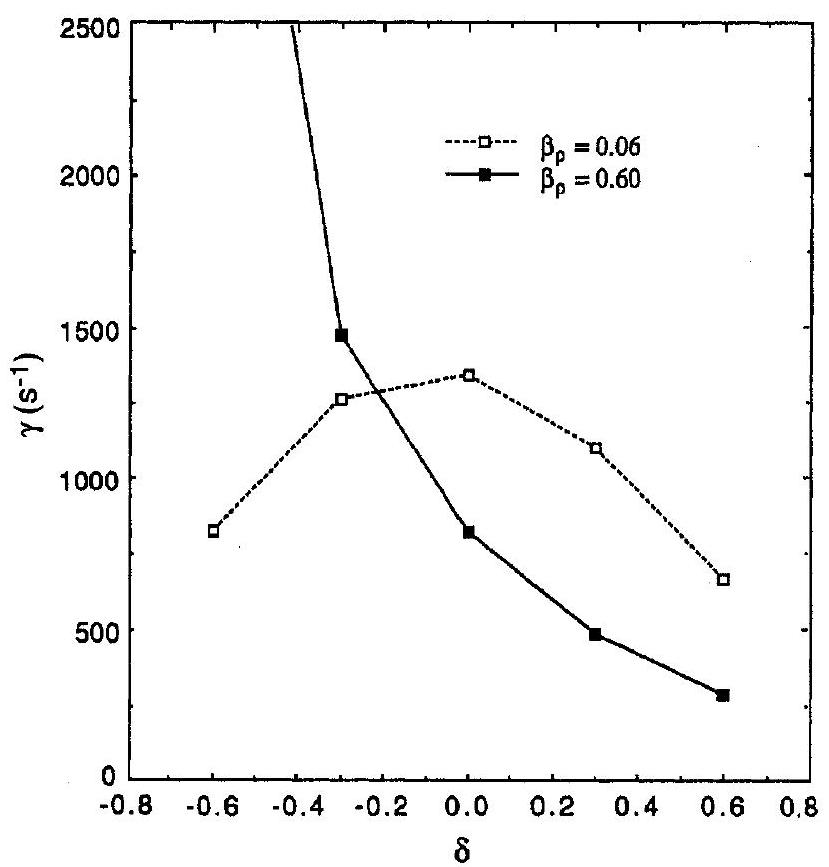
\includegraphics[max width=0.85\textwidth,max height=0.3\textheight]{2025_01_10_a0135324997886412d98g-6}
 \caption{\uline{Growth rates (in $\mathrm{s}^{-1}$ ) versus triangularity for a resistive wall conformal to the plasma shape at a midplane distance of $\mathrm{d}=1.3 \mathrm{a}$ for seversal shapes ranging from the inverse dee $(\delta=-0.6)$ to the regular dee $(\delta=0.6)$ at high beta $\left(\beta_{p}=0.6\right)$ and low beta $\left(\beta_{p}=0.06\right)$.\\}\\在高比压($\beta_{p}=0.6$)和低比压($\beta_{p}=0.06$)条件下,对于从反 D 形($\delta = - 0.6$)到常规 D 形($\delta = 0.6$)的几种形状,与等离子体形状共形且中平面距离为 $\mathrm{d}=1.3 \mathrm{a}$ 的电阻壁的增长率(单位:$\mathrm{s}^{-1}$)随三角形变的变化情况。 }
  	\label{fig4.}
  \end{figure}
  
   \begin{figure}[H]
  	\centering
  	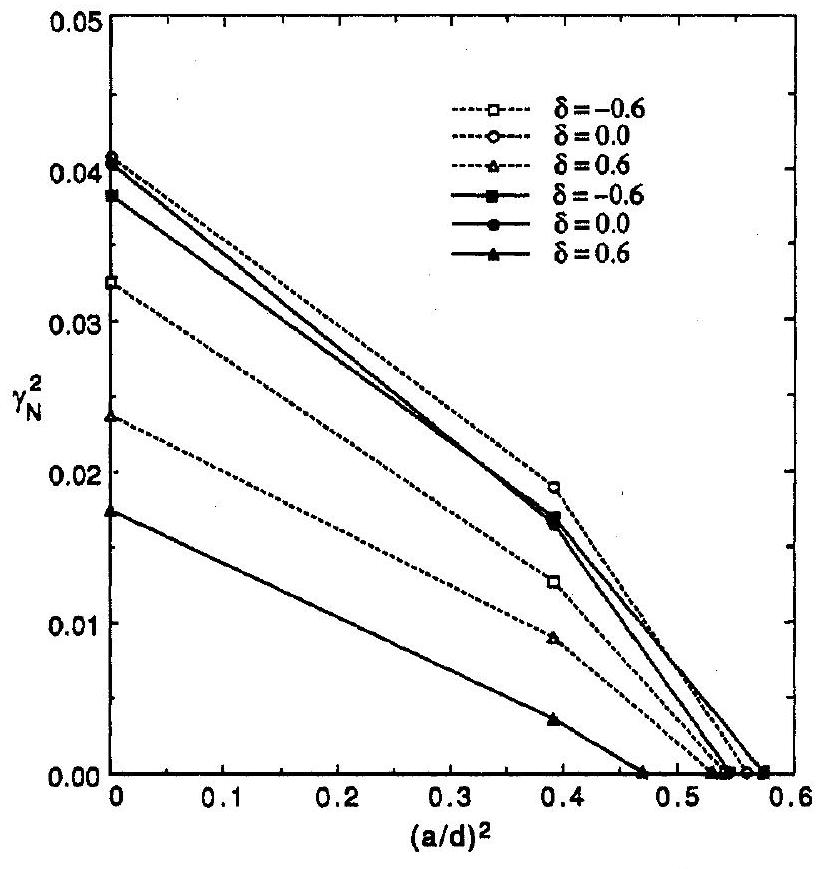
\includegraphics[max width=0.85\textwidth,max height=0.3\textheight]{2025_01_10_a0135324997886412d98g-6(1)}
 \caption{\uline{Plot of the square of the normalized ideal wall MHD growth rate $\gamma_{N}^{2}$ versus $\mathrm{a}^{2} / \mathrm{d}^{2}$, with an ideally conducting wall. The results are shown for three shapes (inverse dee, ellipse, regular dee) at high $\beta_{p}$ (solid symbols) and low $\beta_{p}$ (open symbols).}\\在有理想导电壁的情况下,归一化的理想壁磁流体力学增长率的平方 $\gamma_{N}^{2}$ 与 $\mathrm{a}^{2} / \mathrm{d}^{2}$ 的关系图。图中展示了三种形状(反 D 形、椭圆形、常规 D 形)在高 $\beta_{p}$(实心符号)和低 $\beta_{p}$(空心符号)时的结果。 }
  	\label{fig}
  \end{figure}
 
  
 \section{压强效应}
 {  \small PRESSURE EFFECTS \par }
  
 
\enzhbox{  The operational diagrams in Figs 1 and 3 show a much stronger stabilizing effect of $\epsilon \beta_{\mathrm{p}}$ in the DIII-Dlike cross-section ( $\kappa=2.5, \delta=0.6, \lambda=0$ ) than for the TCV dee shape ( $\kappa=3.0, \delta=0.5, \lambda=0.2$ ).}{
\textcolor{blue}{图 1} 和\textcolor{blue}{图 3} 中的运行图显示,与 TCV D 形($\kappa = 3.0$,$\delta = 0.5$,$\lambda = 0.2$)相比,$\epsilon \beta_{\mathrm{p}}$ 对类似 DIII - D 截面($\kappa = 2.5$,$\delta = 0.6$,$\lambda = 0$)的稳定效应要强得多。 }
  
 
\enzhbox{  Figure 3 shows that the most important reason for this difference is the more triangular shape of DIII-D (note that a positive $\lambda$ decreases the effective triangularity \textcolor{green!50!black}{[9]}). The strong dependence of the pressure effect on triangularity is illustrated by Fig. 4. This figure shows resistive wall growth rates for elongated crosssections ( $\kappa=2.5, A=3$ ) at low and high pressures ( $\beta_{p}=0.06$ and 0.6 , respectively) and at several different triangularities ranging from $\delta=-0.6$ (inverse dee) to $\delta=+0.6$ (standard dee). The wall is a conformal copy of the plasma surface with minor radius $d=1.3 a$ and has the same resistivity and thickness as the TCV vacuum vessel used for Fig. 1. Pressure is strongly destabilizing for the inverse dee, somewhat stabilizing for the ellipse and clearly stabilizing for the standard dee. The inverse dee is strongly destabilized, and with $\beta_{\mathrm{p}}=0.6$ the mode is near marginal stability with an ideally conducting wall, see Fig. 5.}{
\textcolor{blue}{图 3} 表明,造成这种差异的最重要原因是 DIII - D 的三角形变更明显(注意,正的 $\lambda$ 会降低有效三角形变 \textcolor{green!50!black}{[9]})。\textcolor{blue}{图 4} 展示了压强效应与三角形变的强烈依赖关系。该图给出了拉长截面($\kappa = 2.5$,$A = 3$)在低压和高压(分别为 $\beta_{p}=0.06$ 和 0.6)以及几种不同三角形变(从 $\delta = - 0.6$(反 D 形)到 $\delta = + 0.6$(标准 D 形))下的电阻壁增长率。壁是等离子体表面的共形复制,小半径 $d = 1.3a$,其电阻率和厚度与\textcolor{blue}{图 1} 中所用的 TCV 真空室相同。对于反 D 形,压强具有很强的失稳作用;对于椭圆形,压强有一定的稳定作用;而对于标准 D 形,压强的稳定作用明显。反 D 形会被强烈地致失稳,当 $\beta_{\mathrm{p}} = 0.6$ 时,该模式在有理想导电壁的情况下接近临界稳定状态,见\textcolor{blue}{图 5}。 }
  
 
\enzhbox{  Figure 5 shows the square of the normalized ideal wall MHD growth rate (a measure of the ideal MHD driving energy) versus the reciprocal wall radius squared for three different triangularities ( $\delta=-0.6$, $0.0,0.6$ ) and for both high and low pressures. The dee shape is clearly the most stable among all the cases. For this configuration, a finite pressure is significantly stabilizing in the absence of a wall and remains so when wall stabilization is accounted for.}{
\textcolor{blue}{图 5} 展示了三种不同三角形变($\delta = - 0.6$、$0.0$、$0.6$)以及高低两种压强情况下,归一化的理想壁磁流体力学增长率的平方(理想磁流体力学驱动能量的一种度量)与壁半径倒数的平方之间的关系。显然,在所有情况中,D 形是最稳定的。对于这种位形,在无壁时有限压强具有显著的稳定作用,考虑壁致稳时情况依然如此。 }
  
 
\enzhbox{  By contrast, for the inverse dee, pressure is clearly destabilizing both with and without a wall. The critical wall distance for the inverse dee is quite close to $d=1.3 a$, and therefore the resistive wall growth rate (with the wall at that position) is very large in Fig. 4 for that case. For the pure ellipse, the free space growth rate is virtually the same for the low and high pressure cases, but high pressure shows a stabilizing influence in the presence of a wall, and the growth rate falls below that for the inverse dee as the wall is moved inward.}{
相比之下,对于反 D 形,无论有无壁,压强显然都会导致失稳。反 D 形的临界壁间距非常接近 $d = 1.3a$,因此在\textcolor{blue}{图 4} 中该情况下(壁位于此位置时)的电阻壁增长率非常大。对于纯椭圆形,低压和高压情况下的自由空间增长率实际上是相同的,但在有壁的情况下,高压表现出稳定作用,并且随着壁向内移动,其增长率会降至低于反 D 形的增长率。 }
  
 
\enzhbox{  Plots of the equilibrium flux surfaces show that, for the dee shape, increased pressure reduces the central elongation. This can be interpreted as the result of squeezing in the vertical direction by the combination of triangular shape and the Shafranov shift. The same effect leads to an increased elongation at high $\beta_{p}$ in an inverse dee.}{
平衡磁面图显示,对于 D 形,压强增加会减小中心拉长比。这可以解释为三角形形状与沙弗拉诺夫位移共同作用在垂直方向上挤压的结果。同样的效应会导致在反 D 形中,高 $\beta_{p}$ 时拉长比增大。 }
  
 
 
\enzhbox{  We conclude that the primary effect of pressure on the dee shape is to lower the free space driving energy. Conversely, pressure increases the free space energy for the inverse dee. Thus, the favourable effect of pressure shown in the operational diagrams, Figs 1 and 3 , is mainly due to the lowering of the free space driving energy and not to its effect on the wall coupling. For the ellipse, the free space growth rates are virtually unaffected by pressure, but there is an increase in the wall stabilization for the high pressure case.}{
我们得出结论,压强对 D 形的主要影响是降低自由空间驱动能量。相反,压强会增加反 D 形的自由空间能量。因此,\textcolor{blue}{图 1} 和\textcolor{blue}{图 3} 运行图中显示的压强的有利影响,主要是由于降低了自由空间驱动能量,而不是其对壁耦合的影响。对于椭圆形,自由空间增长率实际上不受压强影响,但在高压情况下壁致稳作用有所增强。 }
  
 \section{电流剖面效应}
 {  \small CURRENT PROFILE EFFECTS \par }
 
\enzhbox{  It is well known that the current profile strongly influences the vertical stability. The almost identical results for different classes of current profiles in Fig. 1 show that the relevant parameter characterizing the current distribution is the internal inductance. Flat current profiles with low internal inductance lead to stronger coupling between the plasma and the external conductors. However, we find computationally that, in the absence of a conducting shell, the growth rate generally increases with decreasing inductance (see also Ref. \textcolor{green!50!black}{[20]}). This is shown in Fig. 6, where the ideal wall growth rate is plotted as a function of the wall radius for two DIII-D shaped equilibria with different internal inductances, $l_{\mathrm{i}}=0.6$ and 0.8 , respectively.}{
众所周知,电流剖面会强烈影响垂直稳定性。\textcolor{blue}{图 1} 中不同类型电流剖面给出的几乎相同的结果表明,表征电流分布的相关参数是内部电感。低内部电感的平坦电流剖面会使等离子体与外部导体之间的耦合更强。然而,我们通过计算发现,在没有导电壳的情况下,增长率通常会随着电感的减小而增大(另见文献 \textcolor{green!50!black}{[20]})。这在\textcolor{blue}{图 6} 中有所体现,\textcolor{blue}{图 6} 绘制了两个具有不同内部电感(分别为 $l_{\mathrm{i}} = 0.6$ 和 0.8)的 DIII - D 形平衡态的理想壁增长率随壁半径的变化关系。 }
  
 
\enzhbox{  Peaking of the current profile is evidently stabilizing when the wall is distant but destabilizing when the wall is sufficiently close. At a wall distance of roughly $d=1.4 a$, the two curves in Fig. 6 cross, and the growth rate is independent of the inductance. This point is close to the critical wall distance. Therefore, the internal inductance has a rather small effect on the marginal position of the ideal wall, but it has a much stronger effect on the resistive growth rates with a close fitting wall \textcolor{green!50!black}{[14]}. In fact, with the wall at $d=1.3 a$, the two cases in Fig. 6 have nearly a factor of two difference in the resistive growth rate. The reduction of the free space growth rate with increasing inductance appears to be due mainly to a reduction of the ellipticity of the central flux surfaces. It should be noted that there are many competing effects, for example a similar reduction of the central triangularity, which reduces the finite pressure stabilization. In addition, peaking of the current profile effectively increases the aspect ratio, so that the toroidal stabilization is reduced. However, as discussed in Section 3, the toroidal stabilization is insignificant for highly elongated cross-sections.}{
当壁较远时,电流剖面的峰化显然具有稳定作用,但当壁足够近时则会导致失稳。在壁间距大约为 $d = 1.4a$ 时,\textcolor{blue}{图 6} 中的两条曲线相交,此时增长率与电感无关。这一点接近临界壁间距。因此,内部电感对理想壁的临界位置影响相当小,但对紧密贴合壁情况下的电阻增长率影响要大得多 \textcolor{green!50!black}{[14]}。实际上,当壁位于 $d = 1.3a$ 处时,\textcolor{blue}{图 6} 中的两种情况在电阻增长率上几乎相差一倍。随着电感增加,自由空间增长率降低似乎主要是由于中心磁面椭圆度的减小。需要注意的是,存在许多相互竞争的效应,例如中心三角形变的类似减小会降低有限压强的稳定作用。此外,电流剖面的峰化实际上会增大环径比,从而降低环向稳定作用。然而,正如第 3 节所讨论的,对于高度拉长的截面,环向稳定作用并不显著。 }
  \begin{figure}[H]
  	\centering
  	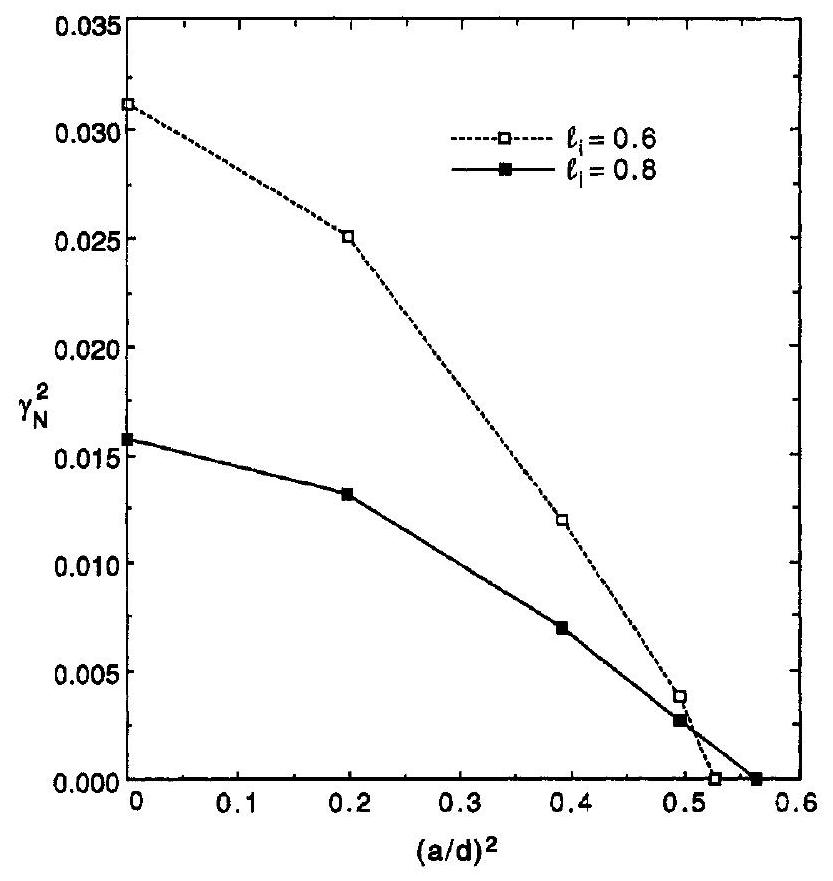
\includegraphics[max width=0.85\textwidth,max height=0.3\textheight]{2025_01_10_a0135324997886412d98g-7}
 \caption{\uline{Plot of $\gamma_{N}^{2}$ versus $\mathrm{a}^{2} / \mathrm{d}^{2}$ with an ideally conducting wall for DIII-D-like equilibria with no pressure for $1_{i}=0.6$ (dashed curve) and for $1_{i}=0.8$ (solid curve).}\\对于无压强的类似 DIII - D 平衡态,绘制有理想导电壁情况下 $\gamma_{N}^{2}$ 与 $\mathrm{a}^{2} / \mathrm{d}^{2}$ 的关系图,其中 $l_{i}=0.6$ 对应虚线曲线,$l_{i}=0.8$ 对应实线曲线。 }
  	\label{fig6.}
  \end{figure}
  
   
 \subsection{离散导体的被动致稳}
 {  \small Passive stabilization by discrete conductors \par }
 
\enzhbox{  While the effect of broadening the current profile increases the destabilizing force on the equilibrium, it also increases the stabilizing effect of a completely surrounding conducting wall. The balance between these competing effects is changed if the passive stabilization is provided primarily by discrete conductors instead of a complete, surrounding wall. As an example, we consider the configuration indicated in Fig. 7. The equilibrium has $\kappa=1.9, \delta=0.7$ and $A=4.54$. Figure 8 shows that in this configuration the growth rate increases with decreasing $l_{\mathrm{i}}$. This effect has been observed previously by Pearlstein \textcolor{green!50!black}{[23]} and by Jardin \textcolor{green!50!black}{[24]}.}{
虽然展宽电流剖面的效应会增加平衡态的失稳力,但它也会增强完全包围等离子体的导电壁的稳定作用。如果被动致稳主要由离散导体而非完整的包围壁提供,那么这些竞争效应之间的平衡就会改变。例如,我们考虑\textcolor{blue}{图 7} 所示的位形。该平衡态的 $\kappa = 1.9$,$\delta = 0.7$,$A = 4.54$。\textcolor{blue}{图 8} 显示,在这种位形下,增长率随 $l_{\mathrm{i}}$ 的减小而增大。珀尔斯坦 \textcolor{green!50!black}{[23]} 和贾尔丁 \textcolor{green!50!black}{[24]} 此前已观察到这种效应。 }
  
 
\enzhbox{  An interesting comparison is obtained by replacing the discrete conductors by the complete wall, as indicated by a dotted contour in Fig. 7. The total wall resistance was normalized to that of the passive conductors. Figure 8 shows that with the closed wall configuration the growth rate decreases monotonically with decreasing $l_{\mathrm{i}}$.}{
通过用完整的壁替代离散导体(如\textcolor{blue}{图 7} 中虚线轮廓所示),可以得到一个有趣的对比结果。将整个壁的电阻归一化为被动导体的电阻。\textcolor{blue}{图 8} 显示,在封闭壁位形下,增长率随 $l_{\mathrm{i}}$ 的减小而单调降低。 }
  
 
\enzhbox{  Figure 7 shows the contours of perturbed flux for the cases of (a) high and (b) low $l_{\mathrm{i}}$ in Fig. 8. While the coupling of the perturbed flux to the closed wall is   improved in the low $l_{i}$ case, the coupling to the discrete conductors is not. Therefore, the increase in the destabilizing force due to the broader current profile dominates, and the growth rate increases with decreasing $l_{\mathrm{i}}$.}{
\textcolor{blue}{图 7} 展示了\textcolor{blue}{图 8} 中(a)高 $l_{\mathrm{i}}$ 和(b)低 $l_{\mathrm{i}}$ 情况下的扰动磁通量等值线。虽然在低 $l_{\mathrm{i}}$ 情况下,扰动磁通量与封闭壁的耦合得到改善,但与离散导体的耦合并未改善。因此,由更宽的电流剖面导致的失稳力增加占主导地位,增长率随 $l_{\mathrm{i}}$ 的减小而增大。 }
  \begin{figure}[H]
  	\centering
  	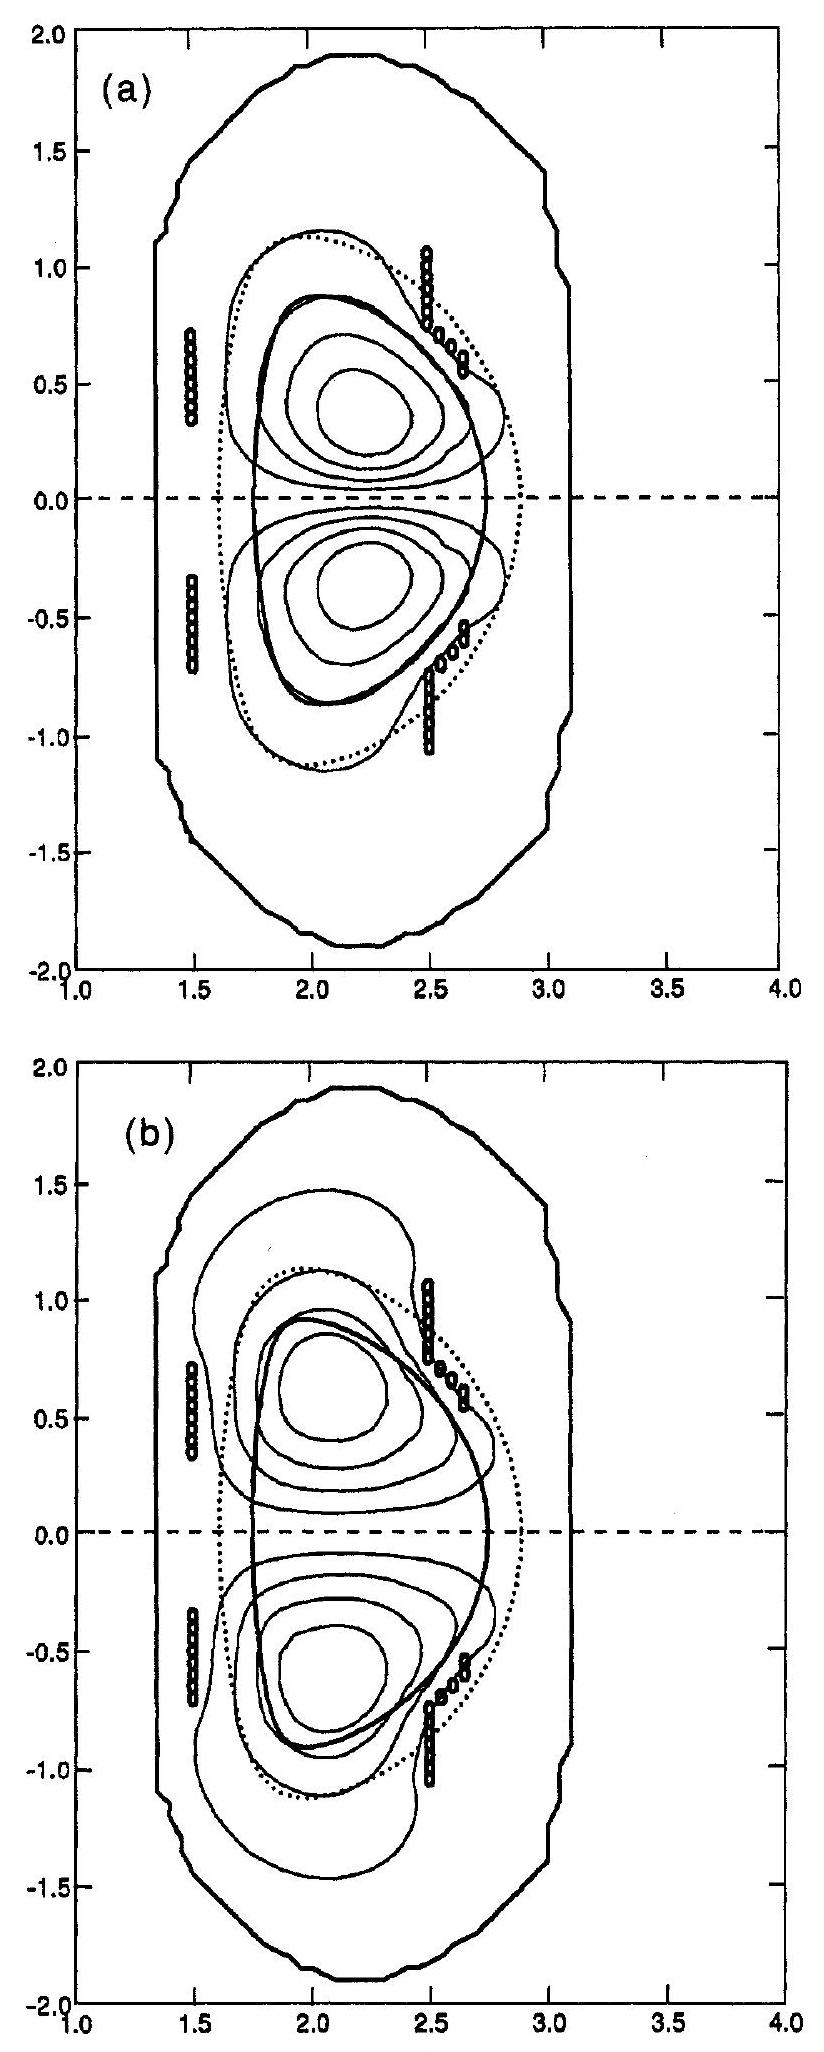
\includegraphics[max width=0.85\textwidth,max height=0.5\textheight]{2025_01_10_a0135324997886412d98g-8(1)}
 \caption{\uline{The plasma boundary, the discrete conductor sets and (shown as a dotted contour) a fictitious completely surrounding wall for the comparison in Fig. 8. The vacuum vessel is quite distant from the plasma. The perturbed flux contours are shown for two equilibria with (a) high $1_{i}$ and (b) low $1_{i}$ in the configuration with discrete conductors.\\}\\图中展示了等离子体边界、离散导体组,以及(以虚线轮廓表示)用于\textcolor{blue}{图 8} 对比的假想的完全包围壁。真空室与等离子体相距较远。图中给出了在离散导体位形下,两个平衡态(a)高 $l_{i}$ 和(b)低 $l_{i}$ 时的扰动磁通量等值线。 }
  	\label{fig7.}
  \end{figure}
  
   \begin{figure}[H]
  	\centering
  	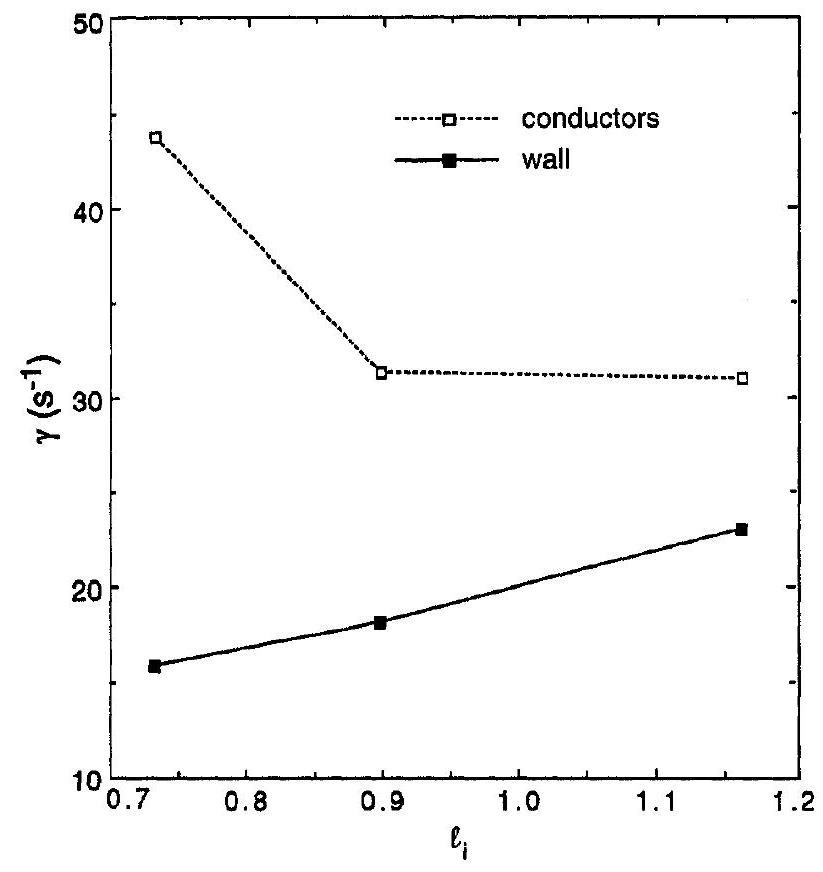
\includegraphics[max width=0.85\textwidth,max height=0.3\textheight]{2025_01_10_a0135324997886412d98g-8}
 \caption{\uline{Growth rates (in $s^{-1}$ ) versus $1_{i}$ for the configuration in Fig. 7 stabilized by discrete conductors with the vacuum vessel far from the plasma. For comparison, growth rates are shown with a completely surrounding wall (conformal to the plasma surface at $\mathrm{d}=1.3 \mathrm{a}$ ).\\}\\对于\textcolor{blue}{图 7} 中由离散导体实现稳定且真空室远离等离子体的位形,增长率(单位:$s^{-1}$)随 $l_{i}$ 的变化情况。为作对比,还给出了由完全包围壁(在 $\mathrm{d}=1.3 \mathrm{a}$ 处与等离子体表面共形)实现稳定时的增长率。 }
  	\label{fig8.}
  \end{figure}
  
 
  
 
\enzhbox{  We conclude that, for highly elongated tokamaks, there are two main effects of the internal inductance on vertical stability. Firstly, wall stabilization is improved for low internal inductance because of increased magnetic coupling. Secondly, current peaking reduces the shaping of the internal flux surfaces, which reduces the instability growth rate in the absence of a wall. For highly elongated, feedback stabilized discharges with a closed wall, the effect on wall coupling is more important, and stability improves at low inductance. However, when there is not a completely surrounding wall, the competition of these two effects is more subtle and depends on the details of the current profile and of the placement of the conductors.}{
我们得出结论,对于高度拉长的托卡马克,内部电感对垂直稳定性主要有两个影响。其一,由于磁耦合增强,低内部电感能改善壁致稳效果。其二,电流峰化会减小内部磁面的形变,从而在无壁情况下降低不稳定性增长率。对于有封闭壁且通过反馈实现稳定的高度拉长放电,对壁耦合的影响更为重要,低电感时稳定性会提高。然而,当没有完全包围的壁时,这两种效应之间的竞争更为微妙,且取决于电流剖面的细节以及导体的布置情况。 }
  
 \section{结论}
 {  \small CONCLUSIONS \par }
 
\enzhbox{  We have found that high values of $\epsilon \beta_{\mathrm{p}}$ significantly improve the vertical stability of dee shaped tokamaks.}{
我们发现,较高的 $\epsilon \beta_{\mathrm{p}}$ 值能显著改善 D 形托卡马克的垂直稳定性。}
  
 
\enzhbox{  The effect can be described in terms of an almost linear dependence of the critical internal inductance on $\epsilon \beta_{\mathrm{p}}, l_{\mathrm{i}, \text { crit }} \approx l_{\mathrm{i}, 0}+c \epsilon \beta_{\mathrm{p}}$. Comparison between different cross-sections shows that the coefficient $c$ increases strongly with triangularity and decreases somewhat with elongation. For a DIII-D-like cross-section, the dependence of $l_{\mathrm{i}, \text { crit }}$ on $\epsilon \beta_{\mathrm{p}}$ is quite pronounced. This effect is beneficial for reaching high beta, because it increases the maximum stable elongation or, alternatively, allows the current profile to be more peaked, which increases the beta limit due to the $n=1$ external kink mode $\textcolor{green!50!black}{[2,9]}$.}{
这种效应可以用临界内部电感与 $\epsilon \beta_{\mathrm{p}}$ 近乎线性的依赖关系来描述,即 $l_{\mathrm{i}, \text { crit }} \approx l_{\mathrm{i}, 0}+c \epsilon \beta_{\mathrm{p}}$。不同截面之间的比较表明,系数 $c$ 随三角形变显著增大,随拉长比略有减小。对于类似 DIII - D 的截面,$l_{\mathrm{i}, \text { crit }}$ 对 $\epsilon \beta_{\mathrm{p}}$ 的依赖关系十分明显。这种效应有利于达到高比压,因为它增加了最大稳定拉长比,或者换个说法,允许电流剖面更尖峰化,由于 $n = 1$ 外扭曲模的存在,这会提高比压极限 \textcolor{green!50!black}{[2,9]}。 }
  
 \section{致谢}
 {  \small ACKNOWLEDGEMENTS \par }
 
\enzhbox{  This work was supported in part by the Swiss National Science Foundation. We acknowledge the work of H . Lütjens in adapting the CHEASE equilibrium code for NOVA-W.}{
这项工作部分得到了瑞士国家科学基金会的支持。我们感谢 H. Lütjens 为使 CHEASE 平衡程序适用于 NOVA - W 所做的工作。 }
  \setlength{\parskip}{0pt} \small % ==document body ends
 \section{REFERENCES}
\textcolor{green!50!black}{[1]} TROYON, F., et al., Plasma Phys. Control. Fusion 26 (1984) 209.\\[0pt]
\textcolor{green!50!black}{[2]} LAZARUS, E.A., et al., Phys. Fluids B 3 (1991) 2220; LAZARUS, E.A., et al., Phys. Fluids B 4 (1992) 3644.\\[0pt]
\textcolor{green!50!black}{[3]} YUSHMANOV, P.N., et al., Nucl. Fusion 30 (1990) 1999.\\[0pt]
\textcolor{green!50!black}{[4]} ZAKHAROV, L.E., Sov. Phys. - Tech. Phys. 16 (1971) 645 (English translation: Zh. Tekh. Fiz. 41 (1971) 823).\\[0pt]
\textcolor{green!50!black}{[5]} MUKHOVATOV, V.S., SHAFRANOV, V.D., Nucl. Fusion 11 (1971) 605.\\[0pt]
\textcolor{green!50!black}{[6]} LAZARUS, E.A., et al., Nucl. Fusion 30 (1990) 111.\\[0pt]
\textcolor{green!50!black}{[7]} HOFMANN, F., et al., in Fusion Technology 1986 (Proc. 14th Symp. Avignon, 1986), Vol. 1, Pergamon Press, Oxford (1986) 687.\\[0pt]
\textcolor{green!50!black}{[8]} TAYLOR, T.S., et al., in Plasma Physics and Controlled Nuclear Fusion Research 1990 (Proc. 13th Int. Conf. Washington, DC, 1990), Vol. 1, IAEA, Vienna (1991) 177 ; LAO, L.L., et al., Phys. Fluids B 4 (1992) 232.\\[0pt]
\textcolor{green!50!black}{[9]} ERIKSSON, G., et al., in Plasma Physics (Proc. 1992 Int. Conf. Innsbruck), Vol. 16C, Part I, European Physical Society (1992) 343.\\[0pt]
\textcolor{green!50!black}{[10]} ZARNSTORFF, M.C., et al., in Plasma Physics and Controlled Nuclear Fusion Research 1990 (Proc. 13th Int. Conf. Washington, DC, 1990), Vol. 1, IAEA, Vienna (1991) 109.\\[0pt]
\textcolor{green!50!black}{[11]} LÜTJENS, H., et al., Comput. Phys. Commun. 69 (1992) 287.\\[0pt]
\textcolor{green!50!black}{[12]} WARD, D.J., et al., J. Comput. Phys. 104 (1993) 221.\\[0pt]
\textcolor{green!50!black}{[13]} LAVAL, G., et al., Phys. Fluids 17 (1974) 835.\\[0pt]
\textcolor{green!50!black}{[14]} HANEY, S.W., FREIDBERG, J.P., Phys. Fluids B 1 (1989) 1637.\\[0pt]
\textcolor{green!50!black}{[15]} ERIKSSON, H.G., Plasma Phys. Control. Fusion 34 (1992) 1721.\\[0pt]
\textcolor{green!50!black}{[16]} REBHAN, E., Nucl. Fusion 15 (1975) 277.\\[0pt]
\textcolor{green!50!black}{[17]} REBHAN, E., SALAT, A., Nucl. Fusion 16 (1976) 805.\\[0pt]
\textcolor{green!50!black}{[18]} HOFMANN, F., SCHULTZ, C.G., in Controlled Fusion and Plasma Physics (Proc. 16th Eur. Conf. Venice, 1989), Vol. 13B, Part I, European Physical Society (1987) 335.\\[0pt]
\textcolor{green!50!black}{[19]} BERNARD, L.C., et al., Nucl. Fusion 18 (1978) 1331.\\[0pt]
\textcolor{green!50!black}{[20]} BECKER, G., LACKNER, K., in Plasma Physics and Controlled Nuclear Fusion Research 1976 (Proc. 6th Int. Conf. Berchtesgaden, 1976), Vol. 2, IAEA, Vienna (1977) 401.\\[0pt]
\textcolor{green!50!black}{[21]} STAMBAUGH, R.D., et al., Nucl. Fusion 32 (1992) 1642.\\[0pt]
\textcolor{green!50!black}{[22]} WARD, D.J., JARDIN, S.C., Nucl. Fusion 32 (1992) 973.\\[0pt]
\textcolor{green!50!black}{[23]} PEARLSTEIN, L.D., Lawrence Livermore National Laboratory, personal communication, 1992.\\[0pt]
\textcolor{green!50!black}{[24]} JARDIN, S.C., Plasma Physics Laboratory, Princeton University, personal communication, 1992.\\
(Manuscript received 21 December 1992\\
Final manuscript received 29 March 1993)

  
  	%----------------------------------------------------------------------------------------
  \end{sloppypar}	
  \begin{flushright}
  	\vfill \footnotesize
  	——本翻译PDF由Paper_translator生成, \url{https://github.com/DertahSama/Paper_translator}
  \end{flushright}
  \end{document}
